% In this section the available data sets must be presented. The term dataset
% refers to any type of information source, for example web services for
% geolocation fall into this category. In addition, all necessary data
% manipulation processes, such as cleaning and enrichment with external sources,
% must be presented and discussed.

Il dati sono reperibili direttamente dalla pagina web della challenge; sono
presenti un dataset di train e uno test. Per la valutazione è stato utilizzato
esclusivamente il train in quanto il test è pensato esclusivamente per la
challenge e non contenendo i prezzi target risulta inutile per la valutazione.

Il dataset di train rappresenta quindi il dataset preso in esame e ogni
riferimento successivo al dataset è da intendersi al dataset di train.

Il numero di prodotti contenuti è di circa 1.39 milioni e per ognuno di essi
sono fornite le seguenti caratteristiche.
% assicurarsi che il lettore sia in grado di capire che prodotti sono (già detto
% nell'intro?)

\paragraph{Price} rappresenta il prezzo di vendita dell'articolo, ovvero la
variabile target della regressione. Il suo valore medio è di circa \$26, con un
minimo pari a \$0, un massimo di \$2009 e una deviazione standard di circa \$38.
Analizzando meglio la distribuzione si nota che in generale i prezzi sono
relativamente bassi: inferiori a \$29 per il 75\% dei prodotti.

Dopo aver appreso dal sito ufficiale di Mercari che i prezzi sono impostabili
tra \$5 e \$2000 \cite{mercari-how-to-set-a-price}, sono stati rimossi tutti i prodotti con prezzo minori di 5 e maggiori di 2000.

\paragraph{Train\_id} rappresenta l'identificativo del prodotto nell'elenco.

\paragraph{Name} è il nome del prodotto sotto forma di dato non strutturato.
% todo dato non strutturato. meglio testo?

\paragraph{Shipping} rappresenta di chi, tra venditore e acquirente, sono a carico
le spese di spedizione: il valore 1 significa "a carico del
venditore", 0 invece dell'acquirente.

Il 45\% dei prodotti è spedito a carico del venditore (Shipping=1), mentre il
restante 55\% a carico dell'acquirente (Shipping=0).

Ci si potrebbe aspettare che i prodotti spediti a carico del venditore abbiano
prezzi più elevati; tuttavia  per quanto riguarda il dataset in
esame, è vero il contrario: il prezzo medio dei prodotti spediti a carico degli
acquirenti, circa \$30, è superiore a quello dei prodotti restanti,
circa \$22.

% spese di spedizione sono incluse nel prezzo? todo

\paragraph{Item\_condition\_id} rappresenta lo stato del prodotto; questo valore
varia da 1 a 5. Il valore più frequente è 1, mentre 4 e 5 sono i più rari. La
Kaggle challenge non ne fornisce una descrizione dettagliata del significato. Si
può supporre che il valore 1, il più frequente, identifichi la condizione
migliore, mentre il valore 5 la condizione peggiore. Tuttavia, alla luce dei
prezzi medi per ogni condizione, la supposizione sembra essere errata: i
prodotti in condizione 5 hanno mediamente il prezzo maggiore, quelli in
condizione 4 il minore e le condizioni 1,2,3 hanno prezzo medi molto simili.

% todo dire che abbiamo splittato in 3 le categorie
\paragraph{Category\_name} rappresenta la categoria di prodotto a cui appartiene
l'articolo.

Circa 6000 gli articoli che non hanno nessuna categoria assegnata, mentre i
restanti si suddividono in 1287 categorie, ad esempio \textit{"Women/Tops \&
Blouses/T-Shirts"}, ed è facilmente osservabile una gerarchia di
sottocategorie dalla più generica alla più specifica.


Siccome in più del 99\% dei casi il campo contiene 3 livelli di sottocategorie
il campo \textit{Category\_name} è stato diviso in 3 campi, uno per ogni livello,
assegnando la stringa "NA" a quegli articoli con uno o più livelli mancanti.

\paragraph{Brand\_name} rappresenta il marchio dell'articolo; nel dataset sono
presenti 4809 brand differenti e più di 600 mila valori mancanti: poco meno
della metà dei prodotti totali; a questi prodotti è stato assegnato "NA" come \textit{Brand\_name}.

% todo: scrivere quante parole hanno in media. serve poi nell'embedding? o più
% nel padding del text preprocessing 
\paragraph{Item\_description} rappresenta la descrizione del prodotto sotto forma
di dato non strutturato.

Nel dataset sono presenti 4 istanze senza descrizione e
circa 82 mila con la stringa "no description yet"; in entrambi i casi
\textit{item\_description} è stato impostato a "NA".

Inoltre, non sembra esistere una relazione lineare tra lunghezza delle
descrizioni e prezzo, in quanto l'indice di correlazione di Pearson è prossimo a
zero; 0.048 per l'esattezza.
% todo, omettere? abbiamo calcolato la correlazione solo sulle descrizioni?

Analizzando le word cloud ottenute dai bigrammi delle descrizioni dopo aver
suddiviso i prodotti in quattro fasce di prezzo (figure \ref{fig:100},
\ref{Fig:50_100}, \ref{fig:30_50} e \ref{Fig:minore_30}) si riescono a notare
delle differenze sulle coppie di parole più frequenti, identificabili perchè di
dimensioni più grandi.

Nella wordcloud dei prodotti con prezzo maggiore o uguale a \$100 (Figura
\ref{fig:100}) sono molto frequenti bigrammi che danno informazioni sulle buone
condizioni dei prodotti, ad esempio: "100 authentic", "great condition" e "good
condition". Al diminuire del prezzo questi bigrammi diventano meno frequenti;
aumentano invece i bigrammi relativi a descrizioni mancanti.

\begin{figure}[H]
   \begin{minipage}{0.48\textwidth}
     \centering
     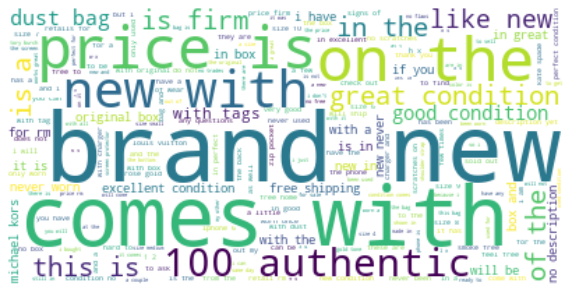
\includegraphics[width=.9\linewidth]{maggiore_100}
	\caption{Descrizioni dei prodotti con prezzo maggiore o uguale a \$100}
	\label{fig:100}   
	\end{minipage}\hfill
   \begin{minipage}{0.48\textwidth}
     \centering
     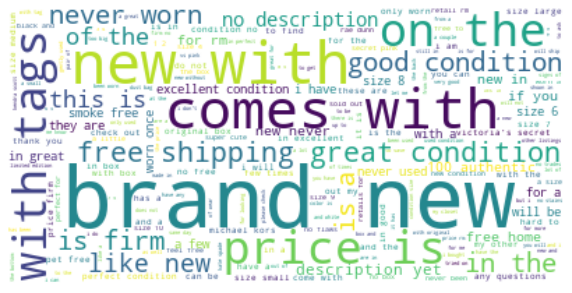
\includegraphics[width=.9\linewidth]{50_100}
     \caption{Descrizioni dei prodotti con prezzo tra \$50 e \$100 esclusi}
     \label{Fig:50_100}
   \end{minipage}
\end{figure}

\begin{figure}[H]
   \begin{minipage}{0.48\textwidth}
     \centering
     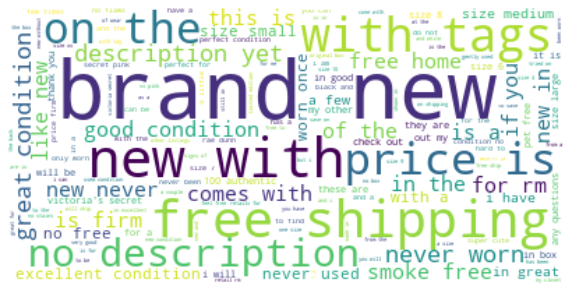
\includegraphics[width=.9\linewidth]{30_50}
	\caption{Descrizioni dei prodotti con prezzo maggiore di \$30 fino a \$50 incluso}
	\label{fig:30_50}   
	\end{minipage}\hfill
   \begin{minipage}{0.48\textwidth}
     \centering
     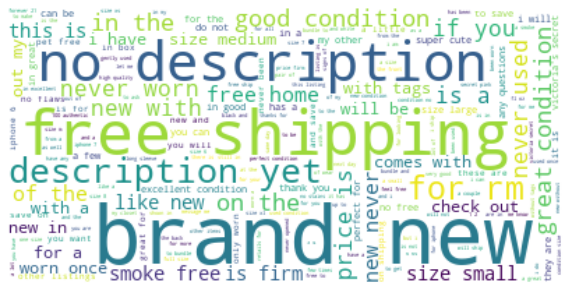
\includegraphics[width=.9\linewidth]{minore_30}
     \caption{Descrizioni dei prodotti con prezzo minore o uguale a \$30}
     \label{Fig:minore_30}
   \end{minipage}
\end{figure}

\subsubsection{Preprocessing del testo}

Il preprocessing del testo è stato effettuato tramite le seguenti operazioni:
\begin{enumerate}
    \item conversione in caratteri minuscoli,
    \item lemmatizzazione,
    \item rimozione della punteggiatura,
    \item rimozione delle \textit{stopwords},
    \item rimozione delle parole di un solo carattere fatta eccezione per i
    numeri la cui rimozione spesso complica la comprensione della descrizione,
    \item rimozione delle emoji.
\end{enumerate}
% in realtà l'orine non è proprio così. cambiare mettendo lemmatizzazione
% all'inizio? todo
In questo lavoro è stato preferito utilizzare la lemmatizzazione poiché usa un
vocabolario per determinare la forma base di una parola, rispetto allo stemming
ovvero un processo euristico che rimuove le estremità delle parole cercando di
ottenere la forma base corretta \cite{balakrishnan2014stemming}. 

Siccome alcuni degli approcci di cui verrà discusso hanno dimostrato performance
migliori con preprocessing limitato a conversione in minuscolo e rimozione della
punteggiatura, in seguito, vi si farà riferimento con preprocessing limitato.
% cito paper sul text preprocessing todo 
% todo cite. Sui dati testuali è stata effettuata una fase di lemmatizzazione (perchè usa
% vocabolario su cui tagliare le parole e cito articolo). Successivamente, sulle

\subsubsection{Encoding}

Per quanto riguarda le variabili categoriche, ovvero \textit{Brand\_name} e le
sottocategorie di \textit{Category\_name},
% todo è chiaro quali sono le
% categooriche? altrimenti chiarire
i valori sono stati codificati in interi tramite \textit{label encoding}.
% todo parlare del label encoding?

I campi testuali invece sono stati codificati in forma vettoriale utilizzando
vari approcci che verranno in seguito discussi.

% tipologie: bow/tfidf, dizionario e poi embedding, tokenizer di bert

% todo: coefficiente di correlazione di  pearson?
% todo: piccole analisi come correlazioni sono da mettere qui? oppure nella
% sezione dopo?
% todo: far trasparire che abbiamo valutato entrambi gli approcci di text
% cleaning o no
